\chapter{Les Chambres à plaques résistives de CMS}
\renewcommand\chapterillustration{RPC/rpc}
\ThisULCornerWallPaper{1}{\chapterillustration}
\minitoc

\lettrine[lines=4, slope=-0.5em]{D}{ans} ce chapitre se veut une description générale des chambres à plaques résistive (RPC) ainsi qu'une description détaillée des chambres RPC utilisées dans CMS ainsi que de leurs électronique. Une description des mise à niveaux se rapportant à ces détecteurs, notamment dans les bouchons sera également présentée.

\section{Les chambres à plaques résistives (RPC)}

 \marginpar
{
	\centering
	\includegraphics[width=\marginparwidth]{RPC/Geiger.png}
	\captionof{figure}{Photo d'un des premiers tubes Geiger-Muller fabriqué en 1932 par Hans Geiger pour une utilisation en laboratoire.}
	\label{Geiger}
}
Les RPC pour \textit{Resistive Plate Chambers} font partie d'une famille de détecteurs appelé détecteur gazeux. Ces détecteurs ont joué un rôle dès le début de la Physique de Haute Énergie dans la détection de nouvelle particules. Depuis le premier détecteur gazeux, le compteur proportionnel à un seul fil \textit{Single-wire proportional counter} inventé par Rutherford et Geiger, puis le compteur Geiger-Mueller (cf.fig\ref{Geiger}) présenté en 1928, les détecteurs gazeux n'ont cessé de se perfectionner et devenir plus rapide, efficaces et permettent de couvrir de grande surface de détections à des coûts très modestes.

\subsection{Les détecteurs gazeux}
Les détecteurs gazeux repose tous sur le même principe simple. Lorsqu'une particule traverse un gaz, elle l'ionise. Les ions et électrons créés lors de cette ionisation peuvent être accéléré grâce à une champ électrique. En choisissant judicieusement l'intensité du champ électrique, c'est à dire en appliquant une tension aux bornes des électrodes, les électrons peuvent gagner assez d'énergie pour ionisé le gaz à leur tours (seconde ionisation) et commencé une multiplication de charge. Le nombres de charge libéré détermine le mode de fonctionnement du détecteur. Le gas est également un élément important du détecteur est à un rôle important sur le mode de fonctionnement de celui-ci. Le déplacement des ces charges à l'intérieur du gaz induit un déplacement de charges sur les électrodes, et crée un signal qui peut être récupéré par une électronique et donner une information sur le temps et la position de la trajectoire de la particule incidente. Ces charges peuvent donner lieux à un mode dit "streamer" voir donner lieux à la création d'étincelles entre l'anode la cathode. La figure \ref{mult} montre le facteur d'amplification, ou le gain du gas en fonction du voltage appliqué. 

\begin{figure}[h!]
	\centering
	\includegraphics[width=0.95\textwidth]{RPC/gasgain.png}
	\captionof{figure}{Evolution typique de gain du gaz zn fonction du voltage appliqué (en échelle arbitraire).}
	\label{mult}
\end{figure}

Six régions peuvent être définies :

\begin{itemize}
	\item \textbf{I} Les paires d'électrons-ions primaires se recombine avant d'avoir le temps de produire une seconde ionization.
	\item \textbf{II} Les charges du à l'ionization primaire sont entièrement récolté sur les électrodes. Le facteur d'amplification reste constant même si le voltage est augmenté.
	\item \textbf{III} Les charges produitent par l'avalanche sont proportionnel au charges produitent lors de la première ionisation. Les charges colléctés augmentent fortement avec la tension appliqué.
	\item \textbf{IV} Cette région est la limté de proportionnalité, l'avalanche se transforme en streamer, un plasma d'ions et d'électrons.
	\item \textbf{V} Les streamers connectent les électrodes et produissznr des étincelles visible. Les compteur Geiger-Muller et les chambres à étincelles fonctionnent dans ce mode.
	\item \textbf{VI} Des décharges électrique se produisent même sans le passage de particules pour ioniser le gaz. Ce mode peut détruire le détecteur.
\end{itemize}

Les détécteur gazeux à fils n'ont pas une résolution temporelle de l'ordre de la centaines de nanoseconde. Cela est du au champ électrique de la forme en $\frac{1}{r}$, qui fait que la zone d'amplification se situe proche du fil et les électrons doivent atteindre cette zones avant d'être amplifier et de démarrer l'avalanche.

En utilisant un champ électrique uniforme et important, une meilleur résolution temporelle est atteignable.

Le premier détecteur gazeux utilisant cette méthode est le compteur à étincelle "Spark Counter" développé dans les années 1948 , un détecteur qui présente une géométrie plane. Il est généralement constitué de deux électrode métalliques entre lequel est présent un gaz. Le passage d'une particule ionise ce gaz et crée une avalanche qui rentre à un certain moment en mode streamer. Un plasma se créent entre les deux électrodes, les électrodes se déchargent et amène à la création d'une étincelle. Ce type de détecteur présente un signal qui ne nécessite pas d'amplification, cependant le temps nécessaire à le recharge des electrodes est de l'ordre de quelques millisecondes. De plus la surface du détecteur ne doit pas être trop grande (~cm2) afin de ne pas détruire les électrodes lors des décharge.

Afin de résoudre ces problème, les électrodes métalliques peuvent être remplacés par des plaques de matèriaux de hautes résistivité ($10^{9}$ à $10^{10}$ohms) afin de limité l'aire de décharge des électrodes autour du signal ainsi qu'une mélange de gaz absorbant les photons afin d'éviter le mode streamer. Ce qui permet le fonctionnement du détecteur à des flux de particules plus importants et le champs électrics baissant localement du à la recharge plus lentes des électrodes le développement d'avalanches succéssives au même endroit est limités tout en laissant le détecteur opérationnel hors de cette zone.

\subsubsection{Naissance des RPC}
En 1981 R.Santonico et R.Cardarelli développe les Resistive Plate Chamber (RPC). Ce détecteur utilise un matèriaux peu coûteux est très utilisé de haute résistivité (~$10^{10}$ohms), le High Pressure Laminate (HPL) fait de melamine ou phenol resins (Bakelite). Le temps de décharge d'une électrode d'une telle résistivité recevant une charge $Q_{0}$ est donnée par :
\begin{equation}
Q(t)=Q_{0}e^{\frac{-t}{\rho\epsilon_{0}\epsilon_{r}}}
\end{equation}
avec $\rho$ la resistivité volumique du matériaux, $\epsilon_{0}$ la permittivité du vide et $\epsilon_{r}$ la permitivité relative du matériaux.
Les charges présentes sur les électrodes réduisent la haute tension appliqué et donc le champ électrique à l'endroit des charges. Le détecteur devient inefficace pour cette periode de temps $\tau$ à l'endroit du dépot de charge tout en restant efficace ailleurs. Pour de cas du bakelite $\rho\simeq10^{10}ohmscm$ le temps de relaxation de l'ordre de 10ms. Grâce à l'utilisation de matériaux de haute résistivité, l'utilisation de chambres de grande taille était désormais possible.

Plusieurs configuration pour les RPC sont possible, mai l'une des plus simple est donné par la figure \ref{RPCscheme}.

\begin{figure}[h!]
	\centering
	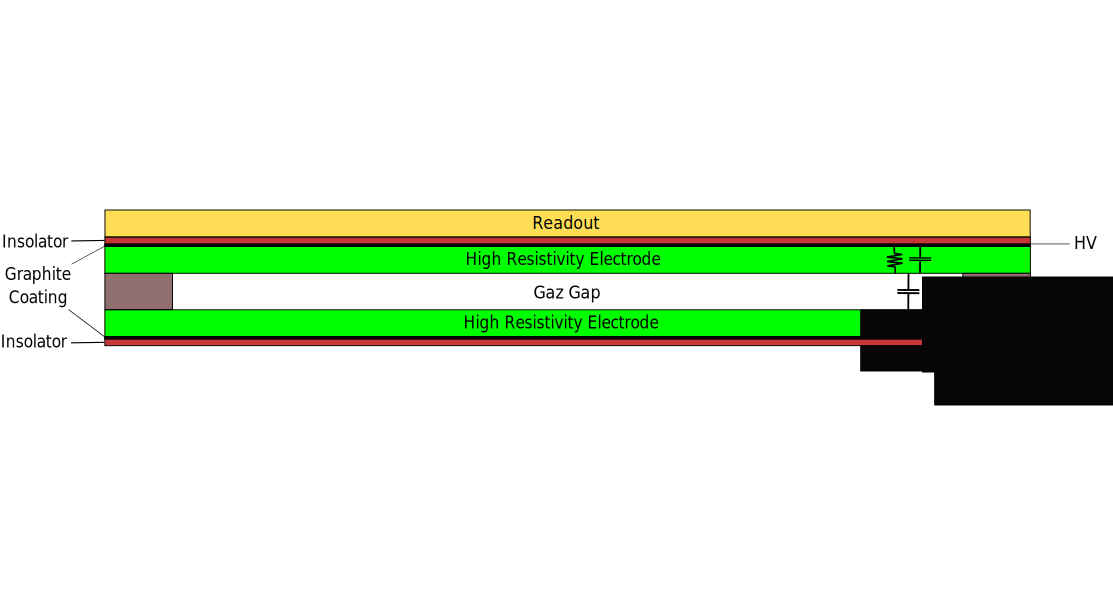
\includegraphics[width=0.98\textwidth]{RPC/scheme_first.png}
	\captionof{figure}{Schéma d'une RPC typique.}
	\label{RPCscheme}
\end{figure}

Une couche de gaz est comprise entre deux plaques d'électrode résistives. Ces plaques sont peintes avec du graphite qui est utilisé pour distribué la haute tension sur les électrodes. Lélectronique est isolée de la chambre par un isolant. L'électronique peut être placé de chaque coté de la chambre et peut être constitué de carreaux ou de lamelles etc.
Depuis ces détecteurs de construction simple et robuste ont été utilisé dans de nombreuses expériences : ATLA, BaBar, BELLE, OPERA etc. Différentes solutions technologiqued ont été développés selon les besoin des différentes expériences.

\subsection{Principes de fonctionnement d'une RPC}
Le principe d'une RPC repose sur l'ionisation d'un gaz. Lorsqu'une particules relativiste traverse le gaz d'une RPC, elle interacgit surtout avec les molécules de gaz par interaction electromagnetique. La perte d'énergie moyenne pour l'ionisation et l'excitation d'une particule relativiste massive ($m>m_{e}$) par des électron libre supposés au repos est donnée par la formule de Bethe-Bloch (cd.fig\ref{Bethe-Block})
\begin{equation}
-\left<\frac{1}{\rho}\frac{\dd E}{\dd x}\right>=\frac{e^{4}}{4\pi \epsilon_{0}^{2}m_{e}c^{2}}z^{2}N_{A}\frac{Z}{A}\frac{1}{\beta^{2}}\left[\frac{1}{2}\ln\frac{2m_{e}c^{2}\beta^{2}\gamma^{2}E_{max}}{I^{2}}-\beta^{2}-\frac{\delta(\beta\gamma)}{2}\right]
\end{equation}
avec :
	\marginpar
{
	\centering
	\includegraphics[width=\marginparwidth]{RPC/Photon.png}
	\captionof{figure}{Émission d'un photon lors de la désexcitation d'un atome.}
	\label{photon}
}
\marginpar
{
	\centering
	\includegraphics[width=\marginparwidth]{RPC/Auger.png}
	\captionof{figure}{Éjéction d'un électron Auger.}
	\label{Auger}
}
\marginpar
{
	\centering
	\includegraphics[width=\marginparwidth]{RPC/Brem.png}
	\captionof{figure}{Bremsstrahlung produit par un muon dévié par le champ électrique d'un noyau.}
	\label{Brem}
}
\marginpar
{
	\centering
	\includegraphics[width=\marginparwidth]{RPC/Penning.png}
	\captionof{figure}{Ionisation Penning.}
	\label{Penning}
}
\begin{itemize}[label=$\bullet$]
	\item $\rho$ la densité du matériaux,
	\item $e$ la charge de lélectron,
	\item $\epsilon_{0}$ la permittivité du vide,
	\item $c$ la vitesse de la umière dans le vide,
	\item $z$ la charge de la particule incidente,
	\item $N_{A}$ le nombre d'Avogadro,
	\item $Z$ le numéro atomique du matériaux,
	\item $A$ le nombre de masse du matériaux,
	\item $\beta=\frac{v}{c}$ la vitesse de la particule incidente en unité de $c$,
	\item $\gamma=\frac{1}{\sqrt{1-\beta^{2}}}$
	\item $I$ est l'énergie d'excitation moyenne et
	\item $E_{max}$ est l'énergie transféré maximale lors d'une collision d'une particule de masse $m$ et de quantité de mouvement $p$,
	\begin{equation}
	\frac{2m_{e}p^{2}}{m^2+2\gamma m_{e}m+m_{e}^2}
	\end{equation}
\end{itemize}

\begin{minipagewithmarginpars}[h]{0.95\textwidth}
	\centering
	\includegraphics[width=0.95\textwidth]{RPC/Bethe-Bloch.eps}
	\captionof{figure}{Perte d'énergie moyenne $-\left<\frac{\dd E}{\dd x}\right>$ pour des anti-muon dans du cuivreen function de $\beta\gamma=\frac{p}{Mc}$ sur neuf ordres de grandeurs en quantité de mouvement (12 ordres de grandeurs en énergie cinétique)\cite{Olive:2016xmw}.}
	\label{Bethe-Block}
\end{minipagewithmarginpars}

Si un atome ou une particule du gaz est ionisé par la collision inelastique de la particule incidente, des électrons sont éjecter de l'atome (la particule) prêt du point de collision. En revanche, si l'atome n'est pas ionisé mais excité, l'énergie d'excitation est évacué par l'émission d'un photon (cf.fig\ref{photon}), par un électron d'Auger (cf.fig\ref{Auger}) ou par ionization Penning (cf.fig\ref{Penning}). Si ce photon à une énergie plus importante que le minimum du potentiel d'ionization, le photon va être absorber par effet photoélectrique est un électron va être éjecté de l'atome, sinon le photon ne sera pas détecter par les RPC.

Une particules chargé relativiste peut aussi perdre son énergie par rayonnement continu de freinage appelé \textit{Bremsstrahlung}(cf.fig\ref{Brem}) , ce processus devient prédominant si l'énergie de la particule dépasse une certaine énergie critique ($E_{\mu c}$ sur la figure \ref{Bethe-Block}).Dans ce cas la perte d'énergie n'est pas détécté par le RPC.

Les RPC repose sur la perte d'énergie par ionisation et excitation. Cette perte d'énergie dépend du matériaux (cf.fig \ref{mat}). Lors de l'ionisation du gaz, des clusters primaires (d'éléctrons et ions ) sont créés le long de la trajectoire de la particule incidentes. 


\begin{figure}[h!]
	\centering
	\includegraphics[width=0.92\textwidth]{RPC/energylost.eps}
	\captionof{figure}{Perte d'énergie moyenne dans l'hydrogène liquide,l'hélium liquide, le carbon, l'aluminium, le fer, l'étain et le plomb. Les effets radiatifs, pertinents pour les pions et muons ne sont pas inclus. Ils deveint important pour les muons traverssant le fer $\beta\gamma\gtrsim1000$ et à plus petite quantité de mouvement pour les muons dans des absorber de plus grand $Z$.\cite{Olive:2016xmw} }
	\label{mat}
\end{figure}

\subsection{Les modes de fonctionnement des RPC}
Selon l'intensité du champ électrique appliqué  entre les électrodes il est possible de choisir le mode de fonctionnement. La composition du mélange gazeux est également un élément déterminant dans le mode de fonctionnement des chambres. On distingue généralement trois modes de fonctionnement; le mode avalanche, le mode streamer et éclair (Spark).

\subsubsection{Le mode avalanche}
Le mode avalanche est le premier mode de fonctionnement qui apparait lorsqu'on augment la tension entre les électrodes.L'ionisation du gaz crée quelques pairs d'ion-électrons qui sont ensuite accéléré par le champ électrique. Les électrons, qui sont beaucoup plus rapides que les ions de par leur masse plus faible vont à leur tours ioniser les molécules du gaz. Cette multiplication des charges est appelée avalanche. Ce déplacement va créée par effet capacitif un signal de l'ordre de la nanoseconde qui peut etre récolter. Les charges vont ensuite atteindre les électrodes et s'y accumuler, et vont être neutraliser en quelques millisecondes grâce au courant fourni par le générateur de haute tension appliquant la différence de potentiel (cf.fig\ref{avalanche}). Le temps mort de ce mode est donc assez faible et permet donc une détection efficace des particules mêle à des flux assez elevée($\sim1kHz$), la résistivité du matériaux est déterminante pour ce temps de neutralisation des charges. Cependant, l a charge induit est faible et nécessite donc une électronique que possédant un bas seuil et donc de bas bruit.


\begin{figure}[ht!]
\centering
\subfloat[Des molècules du gaz sont ionisé par le passage d'une particule.]{\includegraphics[width=.49\linewidth]{RPC/avalanche-streamer-1.png}\label{avalanche-1}}
\hfill
\subfloat[La taille de l'avalanche influence le champ électrique local de la couche de gaz.]{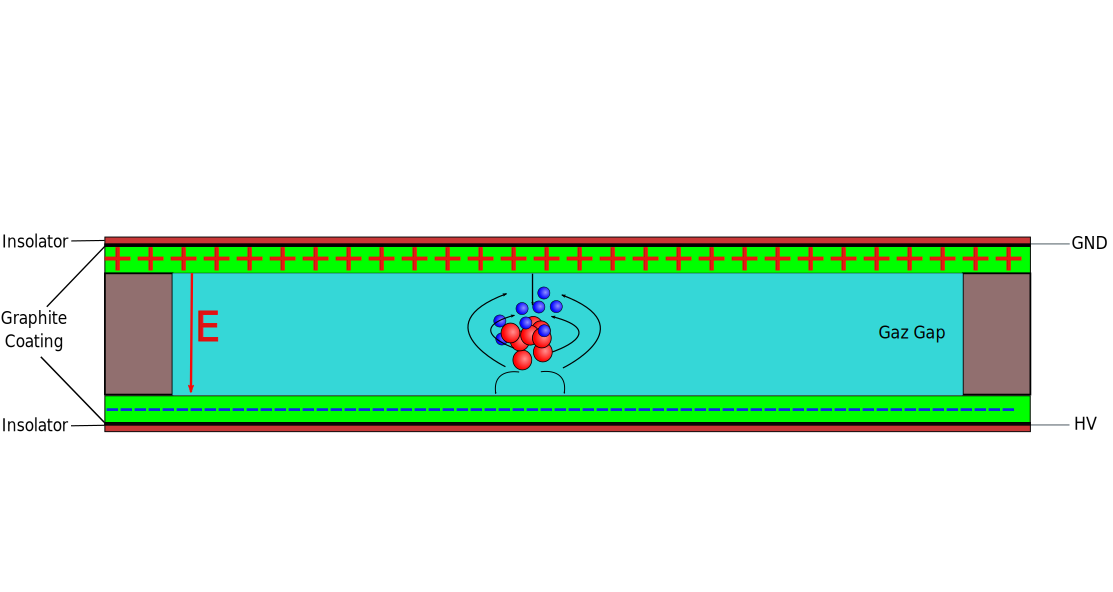
\includegraphics[width=.49\linewidth]{RPC/avalanche-2.png}\label{avalanche-2}}
\\
\subfloat[Les électrons atteignent l'anode. Les ions sont beaucoup plus lent ]{\includegraphics[width=.49\linewidth]{RPC/avalanche-3.png}\label{avalanche-3}}
\hfill
\subfloat[Les ions atteignent la cathode. Les charges de la couche résistive induise un temps mort.]{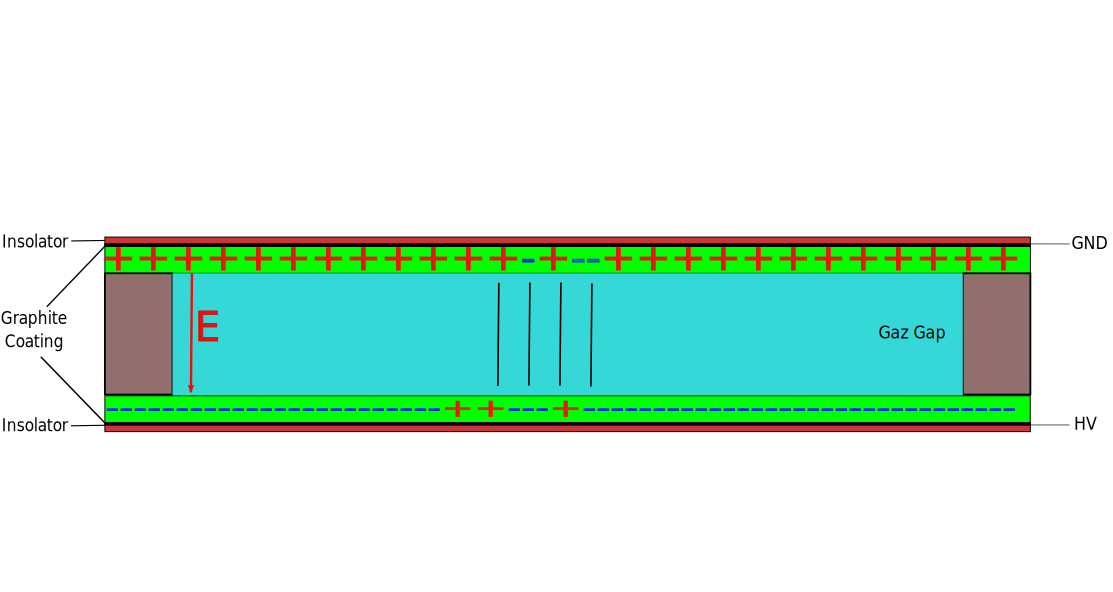
\includegraphics[width=.49\linewidth]{RPC/avalanche-4.png}\label{avalanche-4}}
\caption{Vue schématique d'un développement d'une avalanche. Le champ électrique appliqué au électrode est noté $E_{0}$, les électrons sont en bleu et les ions en rouge.}
\label{avalanche}
\end{figure}

\subsubsection{Le mode streamer}
Si l'on augmente la tension aux bornes des électrodes, le gain du gaz augmente,les ionisation primaires créent donc plus d'ionisation secondaires, il y'a donc création de pairs électrons-ions  en plus grand nombre. De plus les photons peuvent commencer à contribuer à la propagation de l'avalanche, ce qui amène au mode streamer. Le signal engendrer par ce mode est plutôt importannt (de 50pC à quelques nC), l'électronique peut donc se passer d'amplification et est donc beaucoup plus simple. Cependant, le flux de particules maximale est limité à quelques kiloHz. Si le nombre d'électrons devient trop important (en moyenne $10^{8}$ électrons), ils engendre la création d'un plasma reliant les deux électrodes (cf.fig \ref{streamer}).

\begin{figure}[ht!]
	\centering
	\subfloat[Des molècules du gaz sont ionisé par le passage d'une particule.]{\includegraphics[width=.98\linewidth]{RPC/avalanche-streamer-1-2.png}\label{streamer-1}}
	\\
	\subfloat[La taille de l'avalanche modifie fortement le champ électrique local de la couche de gaz. ]{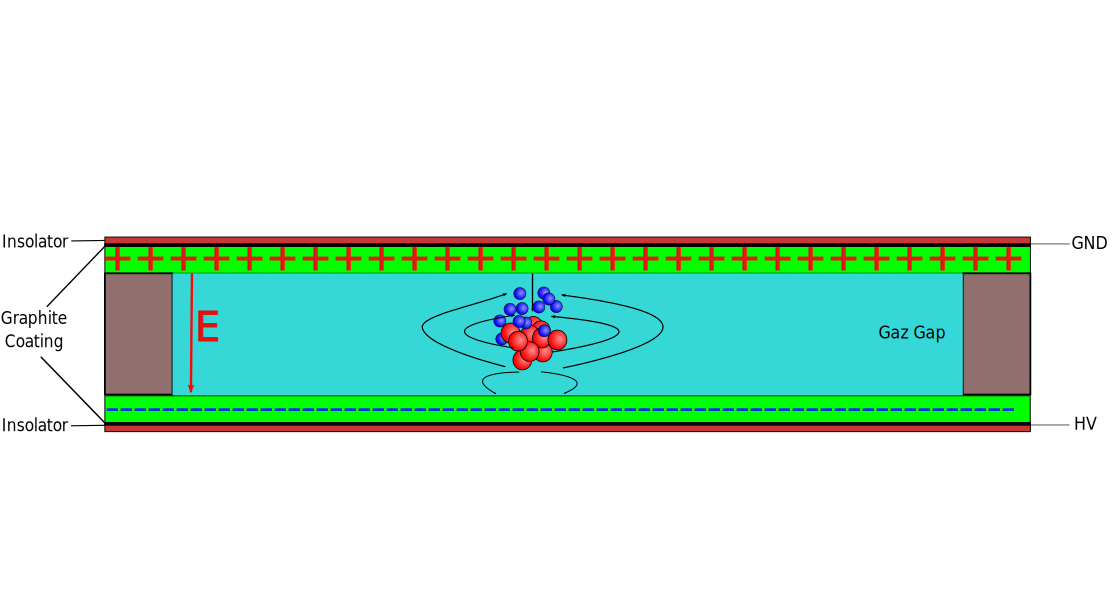
\includegraphics[width=.49\linewidth]{RPC/streamer-2.png}\label{streamer-2}}
	\hfill
	\subfloat[les photons contribuent au développement de l'avalanche et étalent l'avalanche. Passage au mode streamer]{\includegraphics[width=.49\linewidth]{RPC/streamer-3.png}\label{streamer-3}}
	\\
	\subfloat[Un plasma peut se créé entre les électrodes et créer une étincelle. Les electrodes sont décharger à cette endroit (mode éclair).]{\includegraphics[width=.49\linewidth]{RPC/streamer-4.png}\label{streamer-4}}
	\hfill
	\subfloat[Des éclairs se forment de proches en proches à cause des électrons migarteurs et des photons]{\includegraphics[width=.49\linewidth]{RPC/streamer-5.png}\label{streamer-5}}
	\caption{Vue schématique d'un développement d'un streamer. Le champ électrique appliqué au électrode est noté $E_{0}$, les électrons sont en bleu et les ions en rouge.}
	\label{streamer}
\end{figure}

\subsubsection{Le mode éclair (Spark)}
Si l'on augmente encore la tension ou si le mélange de gas ne permet pas de limiter la propagation latérale de l'avalanche ou le mode streamer, les électrons migrateur et les photons peuvent induire de proches en proches d'autres streamers, c'est le mode éclair, ou Spark. Les éclairs se propagent alors dans toute la chambre. Le temps de recouvrement de la chambre est alors très long et les charges accumulé peuvent détériorer raoidement le détecteur. De plus le flux de particules détectable est très faible (cf.fig \ref{spark}).
\begin{figure}[ht!]
	\centering
	\subfloat[Des molècules du gaz sont ionisé par le passage d'une particule.]{\includegraphics[width=.49\linewidth]{RPC/avalanche-streamer-1.png}\label{spark-1}}
	\hfill
	\subfloat[La taille de l'avalanche modifie fortement le champ électrique local de la couche de gaz. ]{\includegraphics[width=.49\linewidth]{RPC/spark-2.png}\label{spark-2}}
	\\
	\subfloat[les photons contribuent au développement de l'avalanche et étalent l'avalanche. Passage au mode streamer]{\includegraphics[width=.49\linewidth]{RPC/streamer-3.png}\label{spark-3}}
	\hfill
	\subfloat[Un plasma peut se créé entre les électrodes et créer une étincelle. Les electrodes sont décharger à cette endroit (mode éclair).]{\includegraphics[width=.49\linewidth]{RPC/streamer-4.png}\label{spark-4}}
    \\
	\subfloat[Des éclairs se crées de proches en proches à cause des électrons migrateurs et des photons.]{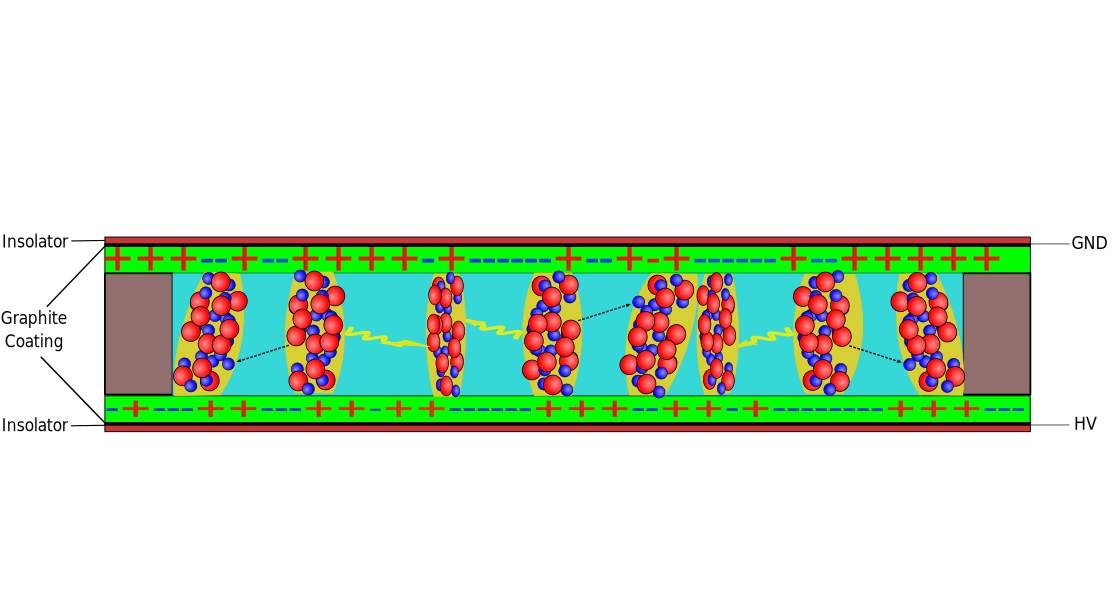
\includegraphics[width=.49\linewidth]{RPC/spark-5.png}\label{spark-5}}
    \hfill
	\subfloat[Le champ électrique est fortement baissé dans toute la chambre; Elle est aveugle.]{\includegraphics[width=.49\linewidth]{RPC/spark-6.png}\label{spark-6}}
	\caption{Vue schématique d'un développement d'un streamer. Le champ électrique appliqué au électrode est noté $E_{0}$, les électrons sont en bleu et les ions en rouge.}
	\label{spark}
\end{figure}


Dans CMS le mélange de gaz ainsi que les tensions appliquées ont été judicieusement étudiées pour que les RPC soient le plsu possible en mode avalanches afin de maximiser le flux de particules que peut détécté les chambres ainsi que d'éviter un vieillisement prématuré de ces chambres. C'est donc ce mode que nous allons étudier plus en avant.

\subsection{Étude théorique du mode avalanche}

\subsubsection{IOnisation primaire}
Le mélange gazeux des détecteurs contient majoritairement un gaz à faible potentiel d'ionisation minimale afin d'être facilement ionisable. En pratique, la plupart des détecteurs utilise du TFE de potentiel d'ionisation minimzl $U_{i}=10.114 \pm0.010eV$ \cite{Chimie:chimie}. La création de charges primaires due au passage d'une particule chargée dans le mélange de gaz est caractérisé par le nombre de clusters moyen créés par unité de longueur ainsi que par le nombres de paires d'électron-ions créées dans chaque clusters.

\subsubsection*{Distance entre les clusters de l'ionisation primaire}
Si l'on considére que l'énergie perdue par dans le matériaux par la particule incidente est négligeable par rapport à son énergie alors les probabilité de collisions ionisante sont indépendant. Les distance entre les clusters de ionisation primaire suivent donc une loi exponentielle :
\begin{equation}
P(z)=\frac{1}{l}\exp\left(\frac{-z}{\l}\right)
\end{equation} 
où $l$ est le libre parcourt moyen et z l'épaisseur à laquelle l'ionisation à lieu en considérant des particules incidentes dont la trajectoire et normal au plan du détecteur. Pour des particule incident d'ngle $\phi$ par rapport à l'axe z la formule devient:
\begin{equation}
P(z)=\frac{1}{\l}\exp\left(\frac{-z}{\cos\phi l}\right)
\end{equation}
La distance moyenne entre clusters primaires peut se calculer en utilisant le programme de simulation Monte-Carlo HEED\cite{HEED}. Une comparaison entre les mesures et les simulations pour l'isobutane et le méthane est donnée fig\ref{lambda} est montre de bon accord\cite{2004NIMPA.518...86R}.  
\begin{figure}[h!]
	\centering
	\includegraphics[width=0.75\textwidth]{RPC/lambda.png}
	\captionof{figure}{Nombre de collision donnant lieux à des ionisation (nombre de clusters) par mm en function de $\gamma-1$, $\gamma=\frac{1}{\sqrt{1-\beta^{2}}}$ pour différent mélanges de gaz, prédit par HEED. $T=296.15K$ et $p=1013mbar$. Les lignes correspondent à des mesures prise de \cite{PhysRevA.6.1507}.  }
	\label{lambda}
\end{figure}

Le nombre  de cluster contenue dans une couche de gaz d'épaisseur $e$ est donc $\bar{n}=\frac{e}{l}$. La probabilité d'avoir $n$ cluster dans cette couche de gaz suis une lois de Poisson :
\begin{equation}
P(n)=\frac{1}{n!}\left(\frac{e}{l}\right)^{n}\exp\left(-\frac{e}{l}\right).
\end{equation}
En supposant un détecteur parfait l'efficacité maximale pour une chambre d'épaisseur $e$ est donné par :
\begin{equation}
\epsilon_{max}=1-P(0)=1-\exp\left(-\bar{n}\right)
\end{equation}
où $P(0)$ est la probabilité qu'aucune ionisation n'est créée dans l'épaisseur de gaz de la chambre.

\subsubsection*{Nombre d'électrons dans les clusters primaires}
Le nombre d'électrons par clusters d'ionisation primaire est variables et dépend de l'énergie échangé entre le gas est la particule incidente. La distribution du "cluster size" a été calculé par Riegler et al. \cite{Riegler:570462} en utilisant HEED pour des mélanges de gaz très utilisé par les RPC (cf.fig\ref{cluster})
\begin{figure}[h!]
	\centering
	\includegraphics[width=0.75\textwidth]{RPC/cluster.png}
	\captionof{figure}{Distribution du cluster size pour deux mélange gazeux typique utilisé par les RPC calculés en utilisant HEED. Les particules incidentes sont des pions de 7 GeV pour le mélange avec 10\% d'isobutane et 120GeV pour le mélange avec 0.3\%. La température du gas est $T=296.15K$ et la pressure $p=1013mbar$. En coupant à 500 électrons le cluster size est de 2.8 pour 0.3\% de SF6.}
	\label{cluster}
\end{figure}

\subsection{Le facteur de multiplication}
Après l'ionisation, les électrons primaires font être accéléré grâce au champ électrique entre les électrodes ce qui peut donner lieux à une avalanche. Cependant afin d'éviter le mode streamer et spark, le mélange gazeux contient généralement des gaz très électronégatifs ce qui à pour éffet de capturer certains électron primaires, les molécule très électronégative ayant tendance à vouloir former des anions, et de réduire ainsi la taille de l'avalanche. 

Tous les électrons non absorbés sont accéléré par le champ électrique et sont soumis à des chocs élastiques et inélastiques avec les autres molécules du gaz. Si l'énergie échangé lors de ces collisions est assez importantes pour ioniser à sont tour d'autres molècules du gaz on assiste à une multiplication des paires électron-ion et à une réaction en cascade.Les électrons migrent vers l'anode et les cations vers la cathode mais à des vitesses beaucoups moins élevé que pour les électrons de par leur masse beaucoup plus importantes. Ces processus ont de très grandes fluctuations stochastiques.

En définissant $\alpha$ le nombre moyen de paire d'ion-électron secondaire créés par unité de distance (coefficient d'ionisation de Townsend) et  $\beta$ représentant le nombre moyen d'électrons capturé par unité de distance par les molécules électronégatives pour former des anions (coefficient d'attachement), il vient pour un déplacement  $\dd x$.
\begin{equation}
	\frac{\dd \bar{n}}{\dd x}=(\alpha-\beta)\bar{n} \quad  \frac{\dd \bar{p}}{\dd x}=(\alpha)\bar{p} 
\end{equation}
avec la première équation la variation du nombre moyen d'électrons et la deuxieme le nombre moyen d'ions positif. On peut définir également $\alpha_{eff}=\alpha-\beta$ qu'on appelle coefficient effectif. En posant $\bar{n}=1$ et $\bar{p}=0$, on obtient le nombre moyens du nombres d'électrons et d'ions positifs produit sur une distance $x$: 
\begin{equation}
\bar{n}=\exp(\alpha-\beta)x \quad \bar{p}=\frac{\alpha}{\alpha-\beta}\left(\exp^{(\alpha-\beta)x}-1\right)
\end{equation}
Le coefficient de Towsend du champ électrique appliqué. La figure \ref{tow} montre cette dépendance pour un mélange de gas.
\begin{figure}[h!]
	\centering
	\includegraphics[width=0.75\textwidth]{RPC/tow.png}
	\captionof{figure}{Coefficient de Towsend et coefficient d'attachement calculé grâce à Imonte \cite{imonte} pour $T=296.15K$ et $p=1013mbar$ pour un mélange de gas particulier \cite[Riegler:570462]. }
	\label{tow}
\end{figure}


\subsubsection{Charge crées par l'avalanche}
La charge totale à la fin du développement du processus de multiplication peut être vu comme la somme de plusieurs avalanches qui sont indépendantes l'une de l'autre. Chaque cluster primaire crée sont avalanches qui est soumises à des fluctuatuions statistique.

En supposant $\alpha$ et $\beta$ constantes, la charge totale à l'emplacement $z$ peut être exprimé comme :
\begin{equation}
q(z)=\sum_{j=1}^{n_c}q_{e}M_{j}n_{j,0}\exp^{(\alpha-\beta)(z-z_O^j)}
\end{equation}
Les fluctuations statistiques sont pris en compte par 4 variables aléatoires :
\begin{itemize}[label=$\bullet$]
	\item Le nombre de clusters $n_c$ qui suit une distribution poissonienne 
	\begin{equation}
	P_{clusters}(n_c=n)=\frac{(\lambda_{eff}d)^{n}}{n!}\exp^{-\lambda_{eff}d}
	\end{equation}
	avec $\lambda_{eff}=\frac{\lambda}{\phi}$ la densité linéaire moyenne de clusters, $\phi$ l'angle d'incidence de la particule incidente et d l'épaisseur de la couche de gaz.
	\item La position $z_0^j$ du cluster $j$ suit la loi Gamma
	\begin{equation}
	P_{j}(z_0^j=x)=\frac{x^{j-1}\lambda_{eff}^{j}}{\Gamma(j)}\exp^{-x\lambda_{eff}} \quad 0<x<d
	\end{equation}
	\item Le nombre d'électrons $n_{0}^{j}$ dans le cluster $j$ suit la loi de distribution trouvé par le programme Heed (cf.fig\ref{cluster}) 
	\item Le facteur $M_{j}$ qui prend en compte les fluctuations de l'avalanche et de la diminution du champ électrique réduit $E/p$ par les ions lors que l'avalanche devient trop importante. Ce facteur est obtenu concrètement en tirant d'une distribution de Polya uen valuer puis en la divisant par le nombre moyens d'électrons de l'avalanche.
\end{itemize}

\subsubsection{Signal induit sur l'électronique}